Throughout the input specification the user is defining variables. As
described in the above sections many of these variables can be
specified by the user to be random variables. The UQ panel is where the user specifies the distribution of these random variables. Besides the properties of random variables, the sampling method and the number of requested samples shall also be defined by the user. The panel is split, as shown
in \Cref{fig:uq_panel}, into two frames:

\begin{enumerate}
\item Sampling Methods 
\item Random Variables
\end{enumerate}

\begin{figure}[!htbp]
  \centering {
    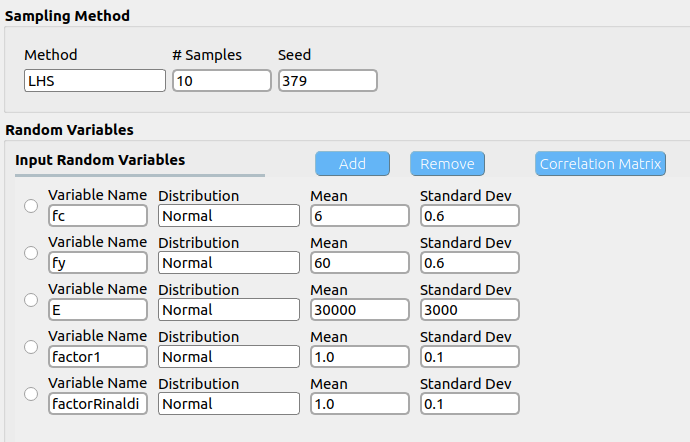
\includegraphics[width=0.8\textwidth]
    {usage/figures/uq1.png} }
  \caption{Uncertainty Quantification input panel}
  \label{fig:uq_panel}
\end{figure}

\subsection{Sampling Methods}
In the forward propagation problem, the user selects the sampling 
method to use from the dropdown menu \href{https://dakota.sandia.gov//sites/default/files/docs/6.9/html-ref/method-sampling.html}{sampling methods}. Currently there are five options available: 
Monte Carlo Sampling (MCS),  Latin Hypercube Sampling (LHS), Importance Sampling (IS), and sampling based on surrogate models, including Gaussian Process Regression (GPR) and Polynomial Chaos Expansion (PCE). Depending on the option selected, the user must specifies the appropriate input parameters for each. For instance, for MCS, the number of samples specifies the number of simulations to be performed, and providing a random seed allows the user to reproduce the same set of samples from the random variables multiple times.

\begin{figure}[!htbp]
  \centering {
    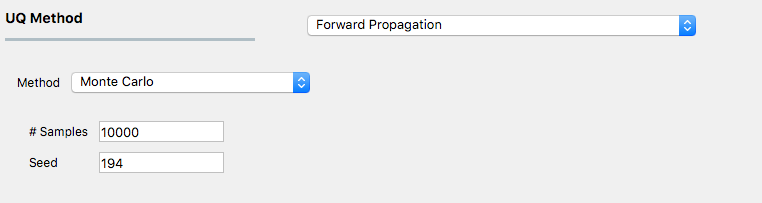
\includegraphics[width=1.0\textwidth]
    {examples/fig_quofem/fw_mc.png} }
  \caption{Monte Carlo Sampling input panel}
  \label{fig:mcs}
\end{figure}

Figure \Cref{fig:mcs} shows the input panel corresponding to the Monte Carlo Sampling (MCS) setting. Two input parameters need to be specified, the number of samples to be executed, as well as the seed used in generating the random samples. 


\begin{figure}[!htbp]
  \centering {
    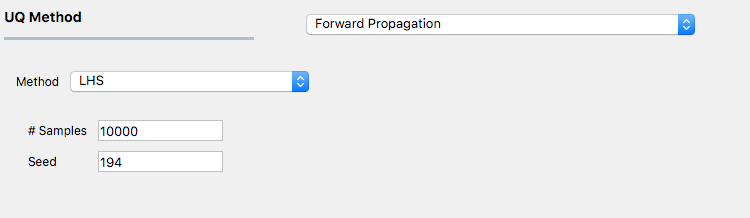
\includegraphics[width=1.0\textwidth]
    {examples/fig_quofem/fw_lhs.png} }
  \caption{Latin Hypercube Sampling input panel}
  \label{fig:lhs}
\end{figure}

Figure \Cref{fig:lhs} shows the input panel corresponding to the Latin Hypercube Sampling (LHS) scheme. Two input parameters also need to be specified, the number of samples to be executed, as well as the seed used in generating the LHS samples. 

\begin{figure}[!htbp]
  \centering {
    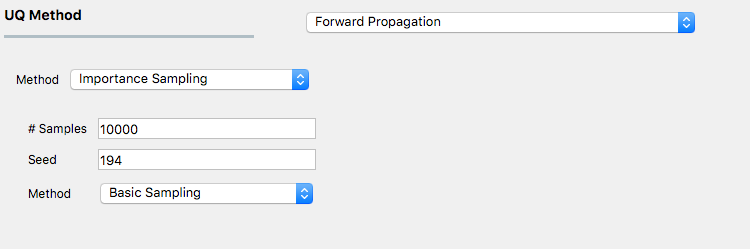
\includegraphics[width=1.0\textwidth]
    {examples/fig_quofem/fw_is.png} }
  \caption{Importance Sampling input panel}
  \label{fig:is}
\end{figure}

For rare event analysis, Figure \Cref{fig:is} shows the input panel for Importance Sampling (IS) scheme. Similar to MCS and LHS, the IS requires both the number of samples to be executed and the corresponding seed for generating such random samples. In addition, the Importance Sampling algorithm can performed via three different approaches, as specified by the third input method. The latter includes Basic Sampling, Adaptive Sampling, and Multimodal Adaptive Sampling. 


For uncertainty propagation with surrogates, two popular surrogates are available, namely Gaussian Process Regression (GPR) and Polynomial Chaos Expansion (PCE). Figure \Cref{fig:gpr} shows the input panel for the GPR model, with input panels for training and sampling. 

\begin{figure}[!htbp]
  \centering {
    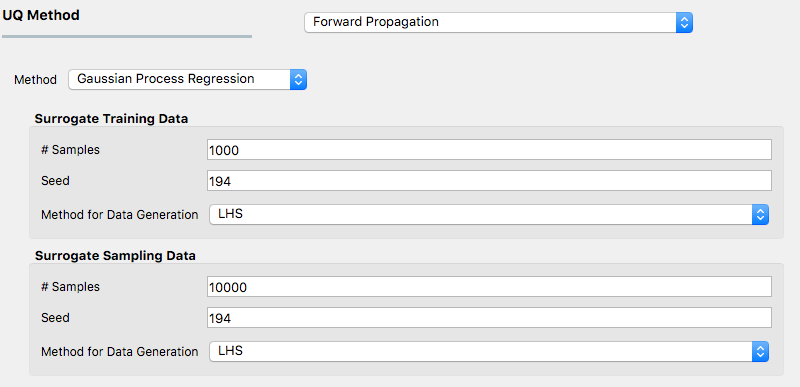
\includegraphics[width=1.0\textwidth]
    {examples/fig_quofem/fw_gp.png} }
  \caption{GPR forward propagation input panel}
  \label{fig:gpr}
\end{figure}

For uncertainty propagation with Gaussian Process Regression (GPR), Figure \Cref{fig:gpr} shows the input panel for the PCE model, with input panels for training and sampling as well. The first set of input parameters in the surrogate training data specify the dataset used for training the surrogate model, while the second set of input parameters in the surrogate sampling data relate to the dataset used for sampling the surrogate. Care must be taken in specifying the training dataset to results in an accurate response surface approximation. 

\begin{figure}[!htbp]
  \centering {
    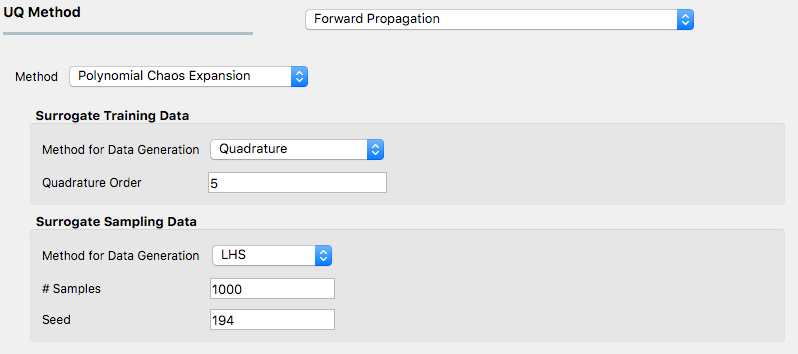
\includegraphics[width=1.0\textwidth]
    {examples/fig_quofem/fw_pce.png} }
  \caption{PCE forward propagation input panel}
  \label{fig:pce}
\end{figure}

For uncertainty propagation with Polynomial Chaos Expansion (PCE), Figure \Cref{fig:pce} shows the input panel for the PCE model, with input panels for training and sampling as well, similar to the input GPR panel. The first set of input parameters in the surrogate training data specify the dataset used for training the surrogate model, while the second set of input parameters in the surrogate sampling data relate to the dataset used for sampling the surrogate. Extreme care must be taken in specifying the parameters of the training dataset to results in an accurate response surface approximation. 

If you are not sure about the training parameters of the surrogates, please refrain from using the surrogates for forward propagation and use instead conventional sampling such as MCS and LHS as discussed above. 

\subsection{Reliability Analysis}

For reliability analysis, figure \Cref{fig:rel} shows the input panel for the reliability capabilities. Currently, both First-Order Reliability Methods (FORM) and Second-Order Reliability Methods (SORM) are supported. The user can specify the local or global solution in the Reliability Scheme input parameter. In addition, the user needs to specify the method for searching for the Most Probable Point (MPP); if not sure, do not use any MPP approximation. 

For both first and second-order reliability analysis, the user needs to specify the either the response levels or the probability levels at which the CDF of the QoI needs to be queried. The user can specify multiple query points, separated by a space. 


\begin{figure}[!htbp]
  \centering {
    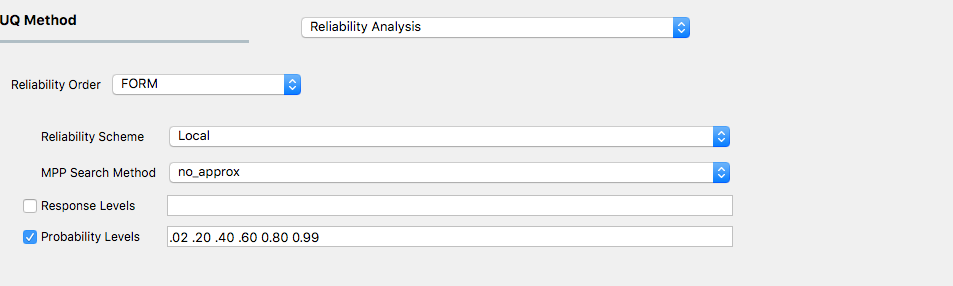
\includegraphics[width=1.0\textwidth]
    {examples/fig_quofem/rel_form.png} }
  \caption{Reliability input panel}
  \label{fig:rel}
\end{figure}




\subsection{Random Variables}
The RV panel allows the user to specify the probabilistic distribution for the random problem at hand. The following probabilistic distributions for the random variables are currently supported: 
\begin{enumerate}
\item Gaussian
\item Lognormal
\item Beta
\item Uniform
\item Weibull
\item Gumbell
\end{enumerate}

Each distribution has different parameters, and the user needs to select accordingly the parameters for the distribution selected for each random variable. Once the user selects the distribution of the random variable, the
corresponding input boxes for the parameters will show. 

\Cref{fig:rv} shows the panel for a problem with four Random Variables with all random input following Gaussian distributions. 

\begin{figure}[!htbp]
  \centering {
    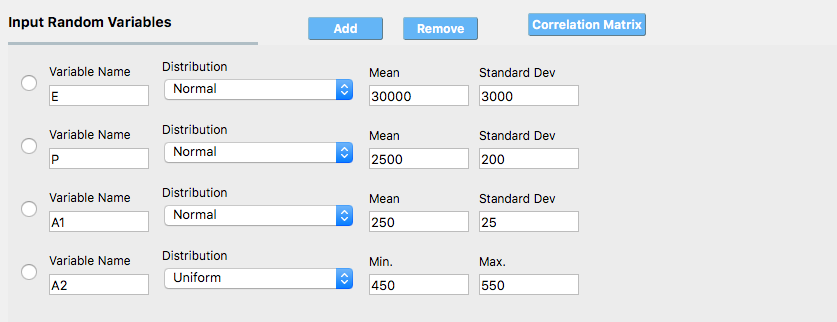
\includegraphics[width=0.8\textwidth]
    {examples/fig_quofem/rv.png} }
  \caption{Random Variable specification}
  \label{fig:rv}
\end{figure}



